\documentclass{beamer}

% Theme and page layout
\usetheme{gapz}
\setbeamertemplate{navigation symbols}{}

% Fonts
\usepackage{fontspec}
\defaultfontfeatures{Mapping=tex-text,Scale=MatchLowercase,Numbers=Lining}
%\setsansfont[
%	ItalicFont = Whitney MediumItalic,
%	BoldFont = Whitney Semibold,
%	BoldItalicFont = Whitney SemiboldItalic,
%	SmallCapsFont = Whitney MediumSC
%]{Whitney Medium}

% Language
\usepackage{polyglossia}
\setdefaultlanguage{english}

% Graphics
\usepackage{graphicx}
\graphicspath{{./images/}}

\title{Three-dimensional modeling and printing project}
\subtitle{Third-year project}
\author[V. Duvert, A. Lubineau, C. Naud, J. Packer, F. Ribon]{\scriptsize
Vincent~Duvert \\ Antoine~Lubineau \\ Caroline~Naud \\ James~Packer \\ Florian~Ribon}
\date{from January 23 to March 16, 2012}

\titlegraphic{
\includegraphics[width=4cm]{inp-enseeiht}}

\begin{document}

\frame{\titlepage}

\section{Presentation of the project}

\subsection{Clients}
\begin{frame}
	\frametitle{Client}
	
	\begin{block}{The \textsc{VORTEX} team}
		\begin{itemize}
			\item Visual Objects from Reality To Expression
			\item still images, video, 2D and 3D scenes
			\item developing methods, models and tools to deal with real or virtual visual objects
		\end{itemize}
    \end{block}
    
    \begin{center}
		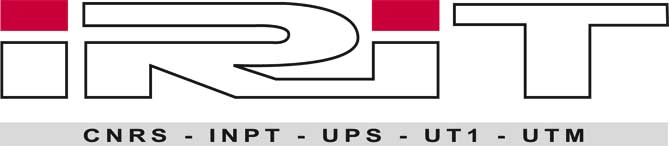
\includegraphics[width=4cm]{irit}
	\end{center}
    
\end{frame}

\subsection{Resources}
\begin{frame}
	\frametitle{Resources}
	
	\begin{block}{Project team}
		\begin{itemize}
			\item several followed the “multimedia” option in third year
		\end{itemize}
    \end{block}
    
    \begin{block}{Material resources}
		\begin{itemize}
			\item an Ultimaker 3D printer
			\item a roll of gray thermoplastic
			\item an Acer T231H touchscreen
			\item a computer
		\end{itemize}
    \end{block}
      
\end{frame}

\begin{frame}
	\frametitle{Ultimaker 3D printer}

    \begin{center}
		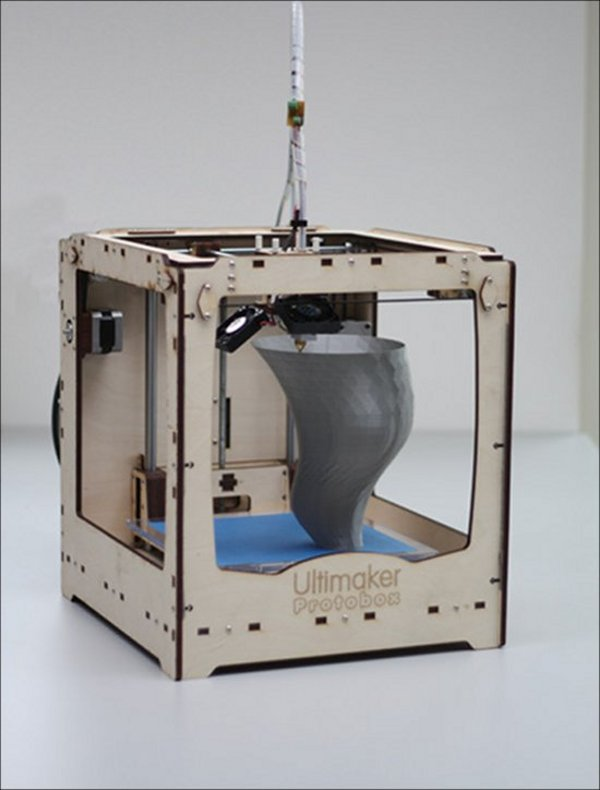
\includegraphics[width=4cm]{Ultimaker}	
	\end{center}
    
\end{frame}

\subsection{Objectives}
\begin{frame}
	\frametitle{blablabla}
    
\end{frame}

\section{Project management}
\begin{frame}
	\frametitle{The V cycle management strategy}

    \begin{center}
		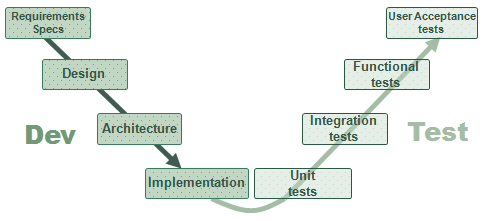
\includegraphics[width=8cm]{VCycle}	
	\end{center}
\end{frame}

\section{Architecture of the project}
\begin{frame}
	\frametitle{blabla}

    \begin{center}
		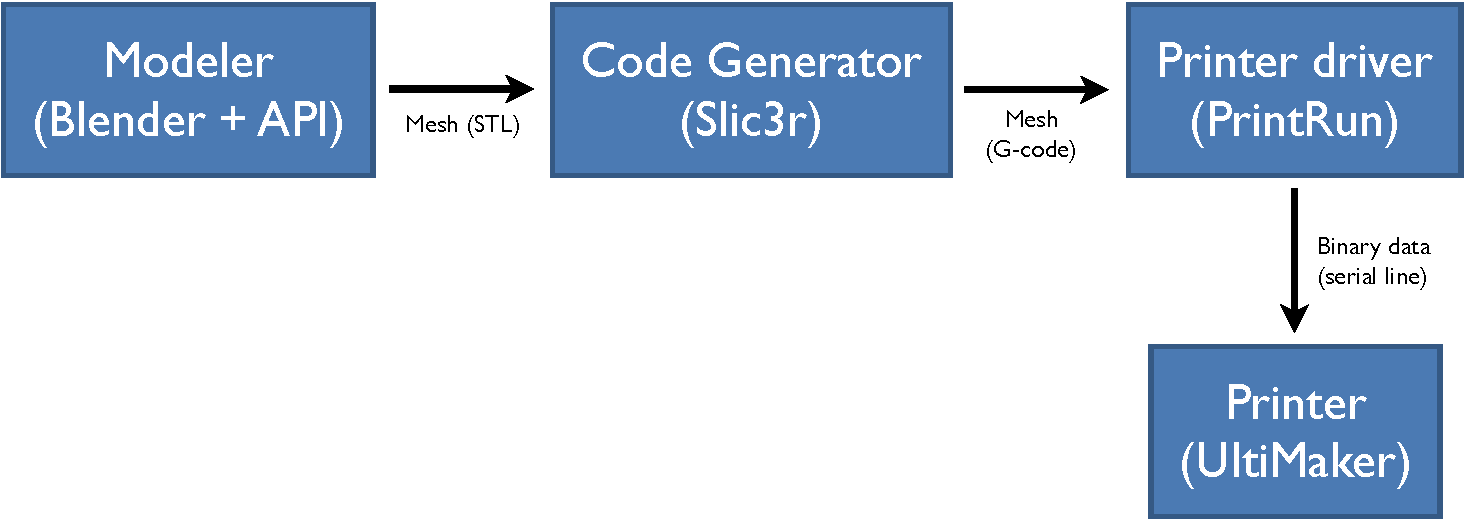
\includegraphics[width=10cm]{schema}	
	\end{center}
	
\end{frame}

\section{Mesh correction}
\begin{frame}
	\frametitle{Mesh correction}

    \begin{block}{Manifold correction}
		\begin{itemize}
			\item manifold checking and hole filling already included in Blender
			\item some bad results
		\end{itemize}
    \end{block}
\end{frame}

\section{Modifications in Blender's interface}
\begin{frame}
	\frametitle{blabla}

    \begin{block}{blabla}
    \end{block}
\end{frame}

\section{Calibration of the printer}
\begin{frame}
	\frametitle{blabla}

    \begin{block}{blabla}
    \end{block}
\end{frame}

\section{Conclusions and thanks}
\begin{frame}
	\frametitle{blabla}

    \begin{block}{blablabla}
    \end{block}
\end{frame}

\begin{frame}
	\frametitle{}

    \begin{center}
    \Large{Thank you for your attention !}
    \end{center}
\end{frame}
	
\end{document}
